\documentclass[12pt]{article}

\usepackage[margin=1in]{geometry}
\usepackage{amsmath,amssymb,amsthm}
\usepackage{graphicx}
\usepackage{booktabs}
\usepackage{hyperref}

\hypersetup{
  colorlinks=true,
  linkcolor=blue,
  citecolor=blue,
  urlcolor=blue
}

\newtheorem{theorem}{Theorem}
\newtheorem{corollary}[theorem]{Corollary}
\newtheorem{remark}{Remark}

\title{IGAD: Information-Geometric Anomaly Detection\\
       via Scalar Curvature of Fisher-Rao Manifolds}

\author{Omry Damari\\
        Independent Researcher\\
        \href{https://github.com/Visigence/IGAD}{https://github.com/Visigence/IGAD}}

\date{2026}

\begin{document}

\maketitle

\begin{abstract}
Classical anomaly detectors based on means, variances, and standard divergences
are blind to distributional shape shifts that preserve the first two moments.
We present \textbf{IGAD} (Information-Geometric Anomaly Detection), a
batch-level anomaly detector whose score is the absolute deviation of the scalar
curvature of the Fisher-Rao statistical manifold between a reference dataset and
an incoming batch:
\[
  \mathrm{IGAD}(\text{batch}) = |R(\theta_{\mathrm{ref}}) - R(\hat{\theta}_{\mathrm{batch}})|
\]
where $R(\theta) = \tfrac{1}{4}(\|S\|^2_g - \|T\|^2_g)$ is the scalar curvature
of the exponential-family manifold at the maximum-likelihood parameter $\theta$,
$S$ is the metric trace vector, and $T$ is the third cumulant tensor contracted
against the Fisher metric $g$.

On the decisive benchmark---Gamma$(\alpha{=}2,\beta{=}1)$ reference vs.\
Weibull (matched mean$=2$, var$=2$) anomaly---IGAD achieves AUC$=0.6199$ at
$n=100$ ($p=0.044$ vs.\ raw skewness) and AUC$=0.6856$ at $n=200$
($p=0.0003$), statistically significantly outperforming both raw skewness and
MLE-skewness baselines. On a pure Dirichlet concentration-profile shift
(identical mean direction, halved $\alpha_0$), IGAD achieves AUC$=0.9999$ at
$n=50$ while MMD reaches only $0.874$ ($p<0.001$, non-overlapping 95\%~CIs).

Our primary contribution is the first use of scalar curvature as a batch-level
anomaly score, together with a mechanistic explanation: the full tensor
contraction of $T_{ijk}$ aggregates $d(d+1)(d+2)/6$ components of the third
cumulant tensor weighted by the inverse Fisher metric, fundamentally different
from any single moment projection. The advantage is most pronounced in the
small-$n$ heavy-tail regime and for higher-dimensional parametric families where
non-parametric methods lack statistical power.
\end{abstract}

\tableofcontents
\newpage

%% ============================================================
\section{Introduction}
%% ============================================================

Anomaly detection is dominated by distance-based and moment-based methods.
Mean-shift detectors, variance-ratio tests, MMD, and Wasserstein distances all
fail on a fundamental class of anomalies: \emph{distributional shape shifts that
preserve mean and variance.} These anomalies arise naturally in practice---a
sensor degradation that changes the tail behavior of a measured quantity without
altering its average or spread, or a physiological transition that changes the
concentration profile of a compositional measurement while preserving its mean
direction.

\paragraph{The matched-moment example.}
Consider two distributions:
\begin{itemize}
  \item \textbf{Reference}: Gamma$(\alpha{=}8,\beta{=}2)$---mean$=4.000$, var$=2.000$, skew$=0.707$
  \item \textbf{Anomaly}: LogNormal$(\mu{=}1.327, \sigma{=}0.343)$---mean$=4.000$, var$=2.000$, skew$=1.105$
\end{itemize}
These distributions are indistinguishable by any test that inspects only location
and scale. Yet their higher-order geometric structure---encoded in the Fisher-Rao
manifold---differs measurably.

\paragraph{This work.}
We propose to use the scalar curvature $R(\theta)$ of the Fisher-Rao statistical
manifold as an anomaly score. The scalar curvature of an exponential family is a
well-defined Riemannian invariant at each parameter point, expressible in closed
form as a quadratic function of the third cumulant tensor. Our detector, IGAD,
computes the MLE parameter estimate $\hat{\theta}$ of each incoming batch and
reports $|R(\theta_{\mathrm{ref}}) - R(\hat{\theta})|$ as the anomaly score.

\paragraph{Key contributions:}
\begin{enumerate}
  \item \textbf{First use of scalar curvature as a batch-level anomaly score} for
        exponential families (Section~\ref{sec:method}).

  \item \textbf{Mechanistic explanation}: the full tensor contraction of $T_{ijk}$
        aggregates all cross-parameter shape channels simultaneously, making the
        curvature estimator more stable than any single scalar projection of the
        MLE parameter (Section~\ref{sec:why-curvature}).

  \item \textbf{Decisive empirical validation}: IGAD beats both raw skewness and
        MLE-skewness at $n=100$--$200$ in the small-$n$ heavy-tail regime with
        $p<0.05$ (Section~\ref{sec:exp-decisive}), and beats MMD and Wasserstein
        on Dirichlet pure-shape shifts with $p<0.001$ at $n=50$
        (Section~\ref{sec:exp-dirichlet}).

  \item \textbf{Honest characterization of failure modes}: Gaussian families
        (constant curvature), 1D families (zero curvature), and large-$n$
        misspecified models are all identified as regimes where IGAD provides no
        advantage (Section~\ref{sec:envelope}).
\end{enumerate}

\paragraph{Summary of key results.}
At $n=100$--$200$, IGAD achieves AUC$=0.62$--$0.69$ in the Gamma vs.\ Weibull
decisive test ($p<0.05$ vs.\ all baselines). For Dirichlet pure concentration
shifts ($k=3,4,5$), IGAD achieves AUC$\geq 0.9999$ at $n=50$ vs.\ MMD AUC of
$0.874$--$0.889$, with $p<0.002$ across all tested configurations.

%% ============================================================
\section{Background and Related Work}
%% ============================================================

\subsection{Fisher-Rao Metric and Exponential Families}

Let $\{p(x;\theta)\}$ be a regular exponential family parameterised by natural
parameters $\theta \in \mathbb{R}^d$:
\[
  p(x;\theta) = \exp\bigl(\langle\theta, T(x)\rangle - A(\theta)\bigr) h(x)
\]
where $A(\theta)$ is the log-partition function. The \textbf{Fisher information
metric} is the Riemannian metric on parameter space defined by the Hessian of
$A$:
\[
  g_{ij}(\theta) = \frac{\partial^2 A}{\partial\theta_i\,\partial\theta_j}
\]
This metric was introduced by Rao~\cite{rao1945} as the natural Riemannian
structure on families of probability distributions, and developed into a full
differential-geometric framework by Amari~\cite{amari1985}. The resulting
geometry is known as \emph{information geometry}.

The \textbf{third cumulant tensor} is the third derivative of $A$:
\[
  T_{ijk}(\theta) = \frac{\partial^3 A}{\partial\theta_i\,\partial\theta_j\,\partial\theta_k}
\]
Both $g$ and $T$ are analytically available in closed form for all standard
exponential families.

\subsection{Scalar Curvature for Hessian Metrics}

Because $g_{ij}$ is the Hessian of a convex function $A$, the Christoffel
symbols simplify to $\Gamma_{ij,k} = \tfrac{1}{2}T_{ijk}$.

A key property of Hessian metrics~\cite{amari2000,ruppeiner1995} is that the
fourth cumulant terms arising in $\partial_i\Gamma^j_{kl}$ are symmetric in
$(i,j)$ but the Riemann tensor is antisymmetric, causing exact cancellation.
The scalar curvature therefore depends \emph{only} on $T$, not on the fourth
cumulant:
\[
  R(\theta) = \tfrac{1}{4}\bigl(\|S\|^2_g - \|T\|^2_g\bigr)
\]
where $S_m = g^{ab}T_{abm}$ is the metric trace vector,
$\|T\|^2_g = g^{ia}g^{jb}g^{kc}T_{ijk}T_{abc}$ is the fully-contracted squared
norm, and indices are raised with the inverse Fisher metric $g^{ij}$.

\subsection{Scalar Curvature in Thermodynamics}

Ruppeiner~\cite{ruppeiner1979,ruppeiner1995} applied scalar curvature of
statistical manifolds to detect phase transitions in thermodynamic systems. In
that setting, $R$ diverges at critical points and encodes correlation structure
of fluctuations. IGAD applies an analogous idea---scalar curvature as a summary
of distributional geometry---but in a fundamentally different domain (batch
anomaly detection) and with a different score construction (deviation rather
than magnitude).

\subsection{Ricci Curvature on Graphs}

A related but distinct line of work~\cite{ollivier2009,lin2011} applies
\textbf{Ricci curvature to graphs} for anomaly detection in network data. This
is a different mathematical object: Ricci curvature there operates on the
topology of a data graph, measuring curvature of optimal transport on the
discrete metric. IGAD operates on the \textbf{Fisher-Rao manifold}---the
geometry of the statistical model itself---and uses \textbf{scalar curvature},
the full Riemann trace, not the Ricci tensor.

\subsection{Two-Sample Tests: MMD and Wasserstein}

The Maximum Mean Discrepancy~\cite{gretton2012} and Wasserstein
distance~\cite{villani2008} are non-parametric two-sample tests that do not
require a parametric family assumption. Their sample complexity is
$O(n^{-1/d})$ for Wasserstein and $O(1/\sqrt{n})$ for MMD, but the constant
factors grow with the intrinsic dimensionality of the distribution. For
correctly-specified parametric families, the MLE converges at the
Fisher-efficient rate $O(1/\sqrt{n})$ with asymptotic variance determined by
the inverse Fisher information---a strictly better constant than kernel-based
estimators at small $n$.

\subsection{Position of IGAD}

IGAD is a \textbf{parametric shape detector}, complementary to non-parametric
methods. It requires a correctly-specified exponential family but, when that
condition is met, achieves parametric sample efficiency for shape detection. It
is not a replacement for MMD or Wasserstein in the large-$n$ regime or when the
family is unknown.

%% ============================================================
\section{Method}
\label{sec:method}
%% ============================================================

\subsection{Exponential Family Setup}

We work with a $d$-dimensional exponential family with log-partition $A(\theta)$.
The key quantities are:
\begin{itemize}
  \item \textbf{Natural parameters}: $\theta \in \mathbb{R}^d$
  \item \textbf{Fisher metric}: $g_{ij} = \partial^2 A/\partial\theta_i\partial\theta_j$ (positive definite)
  \item \textbf{Third cumulant tensor}: $T_{ijk} = \partial^3 A/\partial\theta_i\partial\theta_j\partial\theta_k$ (fully symmetric)
  \item \textbf{MLE}: $\hat{\theta} = \arg\max_\theta \sum_i \log p(x_i;\theta)$
\end{itemize}

For the \textbf{Gamma family} $(\alpha,\lambda)$ with $\lambda=\beta$ the rate
parameter---working in natural parameters $\theta=(\alpha-1,-\lambda)$---the
log-partition is $A(\alpha,\lambda)=\ln\Gamma(\alpha)-\alpha\ln\lambda$,
giving (as implemented in \texttt{igad/families.py}):
\begin{equation}
  g = \begin{pmatrix} \psi_1(\alpha) & 1/\lambda \\ 1/\lambda & \alpha/\lambda^2 \end{pmatrix},
  \label{eq:gamma-metric}
\end{equation}
where $\psi_1(\alpha) = d^2\ln\Gamma/d\alpha^2$ is the trigamma function, and
the non-zero third cumulant entries (up to symmetry) are:
\begin{equation}
  T_{000} = \psi_2(\alpha),\quad
  T_{011} = T_{101} = T_{110} = \frac{1}{\lambda^2},\quad
  T_{111} = \frac{2\alpha}{\lambda^3},
  \label{eq:gamma-T}
\end{equation}
where $\psi_2(\alpha) = d^3\ln\Gamma/d\alpha^3$ is the tetragamma function.
(Note: the off-diagonal $g_{01}=+1/\lambda$ arises in natural parameters
$\theta_2=-\lambda$; in shape-rate parameterisation $(\alpha,\beta)$ the same
entry is $-1/\beta$. The sign convention matches \texttt{GammaFamily.fisher\_metric\_analytical} in \texttt{families.py}.)

For the \textbf{Dirichlet family} $(\alpha_1,\ldots,\alpha_k)$ with
$\alpha_0=\sum_i\alpha_i$~\cite{minka2000}:
\begin{align}
  g_{ij}(\alpha) &= \psi_1(\alpha_i)\,\delta_{ij} - \psi_1(\alpha_0),
  \label{eq:dir-metric} \\
  T_{iii}(\alpha) &= \psi_2(\alpha_i) - \psi_2(\alpha_0),
  \label{eq:dir-T-diag} \\
  T_{ijk}(\alpha) &= -\psi_2(\alpha_0)
  \quad\text{for all $(i,j,k)$ not all equal.}
  \label{eq:dir-T-offdiag}
\end{align}

For the \textbf{Inverse Gaussian family} with natural parameters
$\theta_1 = -\lambda/(2\mu^2)$, $\theta_2 = -\lambda/2$, letting
$a = -\theta_1 > 0$, $b = -\theta_2 > 0$~\cite{folks1978,tweedie1957}:
\begin{align}
  g_{11} &= \frac{\sqrt{b}}{2\,a^{3/2}}, &
  g_{12} &= \frac{-1}{2\sqrt{ab}}, &
  g_{22} &= \frac{1}{2b^2} + \frac{\sqrt{a}}{2\,b^{3/2}},
  \label{eq:ig-metric}
\end{align}
with third cumulant entries:
\begin{align}
  T_{000} &= \frac{3\sqrt{b}}{4\,a^{5/2}}, &
  T_{001} &= \frac{-1}{4\sqrt{b}\,a^{3/2}}, \nonumber\\
  T_{011} &= \frac{-1}{4\sqrt{a}\,b^{3/2}}, &
  T_{111} &= \frac{1}{b^3} + \frac{3\sqrt{a}}{4\,b^{5/2}}.
  \label{eq:ig-T}
\end{align}

\subsection{Scalar Curvature}
\label{sec:curvature}

From the setup in Section~2.2, the scalar curvature at $\theta$ is:
\begin{equation}
  R(\theta) = \tfrac{1}{4}\bigl(\|S\|^2_g - \|T\|^2_g\bigr),
  \label{eq:curvature}
\end{equation}
where:
\begin{align*}
  S_m &= g^{ab}\,T_{abm} = \textstyle\sum_{a,b} g^{ab}\,T_{abm},\\
  \|T\|^2_g &= g^{ia}\,g^{jb}\,g^{kc}\,T_{ijk}\,T_{abc}.
\end{align*}
The formula is $O(d^3)$ to evaluate and is computed analytically for all
supported families, falling back to numerical finite differences otherwise.

\subsection{IGAD Score}
\label{sec:score}

Given a reference dataset $X_{\mathrm{ref}}$ and an incoming batch
$X_{\mathrm{batch}}$:
\begin{enumerate}
  \item Fit $\theta_{\mathrm{ref}} = \mathrm{MLE}(X_{\mathrm{ref}})$ (done once, at fit time).
  \item Compute $R_{\mathrm{ref}} = R(\theta_{\mathrm{ref}})$ (done once).
  \item For each batch $z$: fit $\hat{\theta} = \mathrm{MLE}(z)$, compute
        $R(\hat{\theta})$, return $|R_{\mathrm{ref}} - R(\hat{\theta})|$.
\end{enumerate}
\[
  \boxed{\mathrm{IGAD}(\text{batch}) = |R(\theta_{\mathrm{ref}}) - R(\hat{\theta}_{\mathrm{batch}})|}
\]
Higher scores indicate greater geometric deviation from the reference
distribution. The score is zero when the batch curvature equals the reference
curvature exactly.

\subsection{Why Curvature, Not Skewness}
\label{sec:why-curvature}

A natural question is whether IGAD simply encodes skewness in a roundabout way.
The answer is no, for a structural reason.

\textbf{MLE-skewness} (our primary control) uses the identical MLE parameter
estimate as IGAD but computes only a 1D projection: for Gamma,
$\mathrm{skew}_{\mathrm{MLE}} = 2/\sqrt{\hat{\alpha}}$. This is a single scalar
derived from one component of $\hat{\theta}$.

\textbf{IGAD} computes
$\|T\|^2_g = \sum_{i,j,k,a,b,c} g^{ia}g^{jb}g^{kc}T_{ijk}T_{abc}$, a full
metric-weighted contraction of the $d(d+1)(d+2)/6$ independent components of
$T_{ijk}$. For the Gamma family ($d=2$), these are:
\begin{itemize}
  \item $T_{000} = \psi_2(\alpha)$: the shape channel,
  \item $T_{011} = 1/\lambda^2$: the shape-scale cross-term,
  \item $T_{111} = 2\alpha/\lambda^3$: the scale channel.
\end{itemize}
The cross-term $T_{011}$ encodes the joint co-deviation of $\hat{\alpha}$ and
$\hat{\lambda}$ when the MLE fits misspecified Weibull data. When raw skewness
uses $m_3/m_2^{3/2}$ or MLE-skewness uses $2/\sqrt{\hat{\alpha}}$, this
cross-channel information is discarded. IGAD's tensor contraction aggregates all
channels simultaneously, and noise cancels across channels in a way that it
cannot in any single-channel estimator.

\subsection{Supported Families}

\begin{table}[h]
\centering
\caption{Exponential families supported by IGAD with analytical implementations.}
\begin{tabular}{lcccc}
\toprule
Family & $d$ & Analytical $g$? & Analytical $T$? \\
\midrule
Gamma & 2 & Yes & Yes \\
Dirichlet ($k\geq 3$) & $k-1$ & Yes & Yes \\
Inverse Gaussian & 2 & Yes & Yes \\
Poisson & 1 & Yes & Yes ($R\equiv 0$) \\
Gaussian (fallback) & 3 & Numerical & Numerical \\
\bottomrule
\end{tabular}
\end{table}

%% ============================================================
\section{Theoretical Analysis}
%% ============================================================

\subsection{Asymptotic Variance of the Curvature Estimator}

Let $\hat{\theta}$ be the MLE on $n$ i.i.d.\ samples from the true distribution
$p(\cdot;\theta^*)$. By the delta method:

\begin{theorem}[Asymptotic distribution of the curvature estimator]
\label{thm:delta}
Suppose Assumption~A1 holds (all cumulants of $T(x)$ up to order 5 are finite)
and $\nabla R(\theta^*) \neq 0$. Then
\[
  \sqrt{n}\bigl(R(\hat{\theta}_n) - R(\theta^*)\bigr) \xrightarrow{d}
  \mathcal{N}\!\bigl(0,\,\sigma^2_R(\theta^*)\bigr),
\]
where
\[
  \sigma^2_R(\theta^*) = \bigl(\nabla R(\theta^*)\bigr)^\top
                          \bigl[g(\theta^*)\bigr]^{-1}
                          \bigl(\nabla R(\theta^*)\bigr).
\]
\end{theorem}

\begin{proof}
$R:\Theta\to\mathbb{R}$ is a smooth function of $\theta$ (involving derivatives
of $A$ up to order 3 and $g^{-1}$, all smooth under A1). Apply the multivariate
delta method to $\hat{\theta}_n$ with the function $R$.
\end{proof}

The gradient $\nabla_\theta R$ is expressible in closed form as a combination of
$T_{ijk}$ and the fourth cumulant tensor $Q_{ijkl} = \partial^4 A/\partial\theta_i
\partial\theta_j\partial\theta_k\partial\theta_l$. Crucially, $\sigma^2_R$ is
finite for all regular exponential families~\cite{amari2000}, ensuring that the
curvature deviation estimator is a consistent, asymptotically normal statistic.

\subsection{Detection Power}

The signal-to-noise ratio for detecting a curvature deviation
$\Delta R = |R(\theta_{\mathrm{ref}}) - R(\theta_{\mathrm{anom}})|$ at batch size $n$
is:
\[
  \mathrm{SNR} = \frac{\Delta R \cdot \sqrt{n}}{\sigma_R}
\]
where $\sigma_R = \sigma_R(\theta_{\mathrm{ref}})$ from Theorem~\ref{thm:delta}.
Power grows as $\sqrt{n}$ for fixed $\Delta R$.

\subsection{Sample Complexity Comparison}

By the one-sided normal approximation, IGAD achieves power $1-\beta$ at level
$\alpha$ when $\mathrm{SNR}(n) \geq z_\alpha + z_\beta$. Solving:

\begin{corollary}[Sample complexity of IGAD]
IGAD achieves $80\%$ power at level $5\%$ when
\[
  n \geq (1.645 + 0.842)^2 \cdot \left(\frac{\sigma_R}{\Delta R}\right)^2
    \approx 6.18\,\left(\frac{\sigma_R}{\Delta R}\right)^2.
\]
\end{corollary}

\begin{table}[h]
\centering
\caption{Sample complexity comparison between IGAD and non-parametric baselines.}
\begin{tabular}{lll}
\toprule
Method & Rate & Sample complexity \\
\midrule
IGAD (curvature) & $O(n^{-1/2})$ in param.\ dim $d$ & $O\!\left((\sigma_R/\Delta R)^2\right)$ \\
MMD (Gaussian kernel) & $O(n^{-1/2})$ for fixed kernel & $O(1/\mathrm{MMD}(P,Q)^2)$ \\
Wasserstein ($d$-dim data) & $O(n^{-1/d})$ & $O(\varepsilon^{-d})$ for $d\geq 3$ \\
\bottomrule
\end{tabular}
\end{table}

IGAD's sample complexity $O((\sigma_R/\Delta R)^2)$ depends only on the Fisher
geometry of the model---not on the ambient data dimension. Wasserstein has
complexity $O(\varepsilon^{-k})$ for $k$-dimensional simplex data.

%% ============================================================
\section{Experiments}
%% ============================================================

All experiments are reproducible via the scripts in \texttt{experiments/}. All
results use AUC-ROC with 95\% bootstrap confidence intervals. Statistical tests
use paired sign-permutation tests with 10,000 permutations, one-sided
$H_1$: IGAD $>$ baseline.

\subsection{Experiment 2: Gamma(8,2) vs LogNormal --- Matched Mean and Variance}

\paragraph{Setup.}
Reference Gamma$(8,2)$ vs anomaly LogNormal$(\mu{=}1.327,\sigma{=}0.343)$.
Both have mean$=4.000$ and var$=2.000$ identically. Only higher-order
distributional structure differs (skew: $0.707$ vs $1.105$). Batch size
$n=200$; results averaged over 5 seeds.

\paragraph{Control design.}
To isolate geometry from MLE efficiency, we compare IGAD against the
MLE-skewness control: the identical MLE fit as IGAD, but discarding the
curvature tensor in favour of the scalar projection $2/\sqrt{\hat{\alpha}}$.
If IGAD $\approx$ MLE-skewness, MLE efficiency explains everything. If
IGAD $>$ MLE-skewness, the curvature tensor is doing real work.

\paragraph{Results ($n=200$, 5 seeds).}

\begin{table}[h]
\centering
\caption{Experiment 2 results ($n=200$, 5 seeds). MLE-skewness is the control.}
\begin{tabular}{lcc}
\toprule
Method & Mean AUC & $\pm$Std \\
\midrule
IGAD (curvature) & 0.6542 & 0.047 \\
MLE skewness {[CONTROL]} & 0.6016 & 0.038 \\
MMD (RBF, median BW) & 0.5894 & 0.076 \\
Wasserstein (1D) & 0.5925 & 0.057 \\
Raw skewness & 0.6794 & 0.072 \\
Mean shift {[BLIND]} & 0.5240 & 0.062 \\
Variance shift {[BLIND]} & 0.5818 & 0.027 \\
\bottomrule
\end{tabular}
\end{table}

Gap (IGAD $-$ MLE skewness): $+0.053$. Curvature geometry adds signal beyond
MLE efficiency alone.

\paragraph{Scaling with batch size (seed=42).}

\begin{table}[h]
\centering
\caption{Experiment 2 scaling with batch size (seed=42).}
\begin{tabular}{lcccc}
\toprule
$n$ & IGAD & MLE-skew & Raw-skew & Gap(IGAD$-$MLE) \\
\midrule
100 & 0.5704 & 0.5764 & 0.5908 & $-0.006$ \\
200 & 0.6838 & 0.6098 & 0.6514 & $+0.074$ \\
500 & 0.6748 & 0.5846 & 0.9194 & $+0.090$ \\
1000 & 0.7892 & 0.8214 & 0.9686 & $-0.032$ \\
\bottomrule
\end{tabular}
\end{table}

IGAD beats MLE-skewness at $n=200$ and $n=500$. At $n=1000$, model
misspecification (fitting Gamma to LogNormal) degrades the curvature signal,
and non-parametric methods dominate.

\begin{figure}[h]
\centering
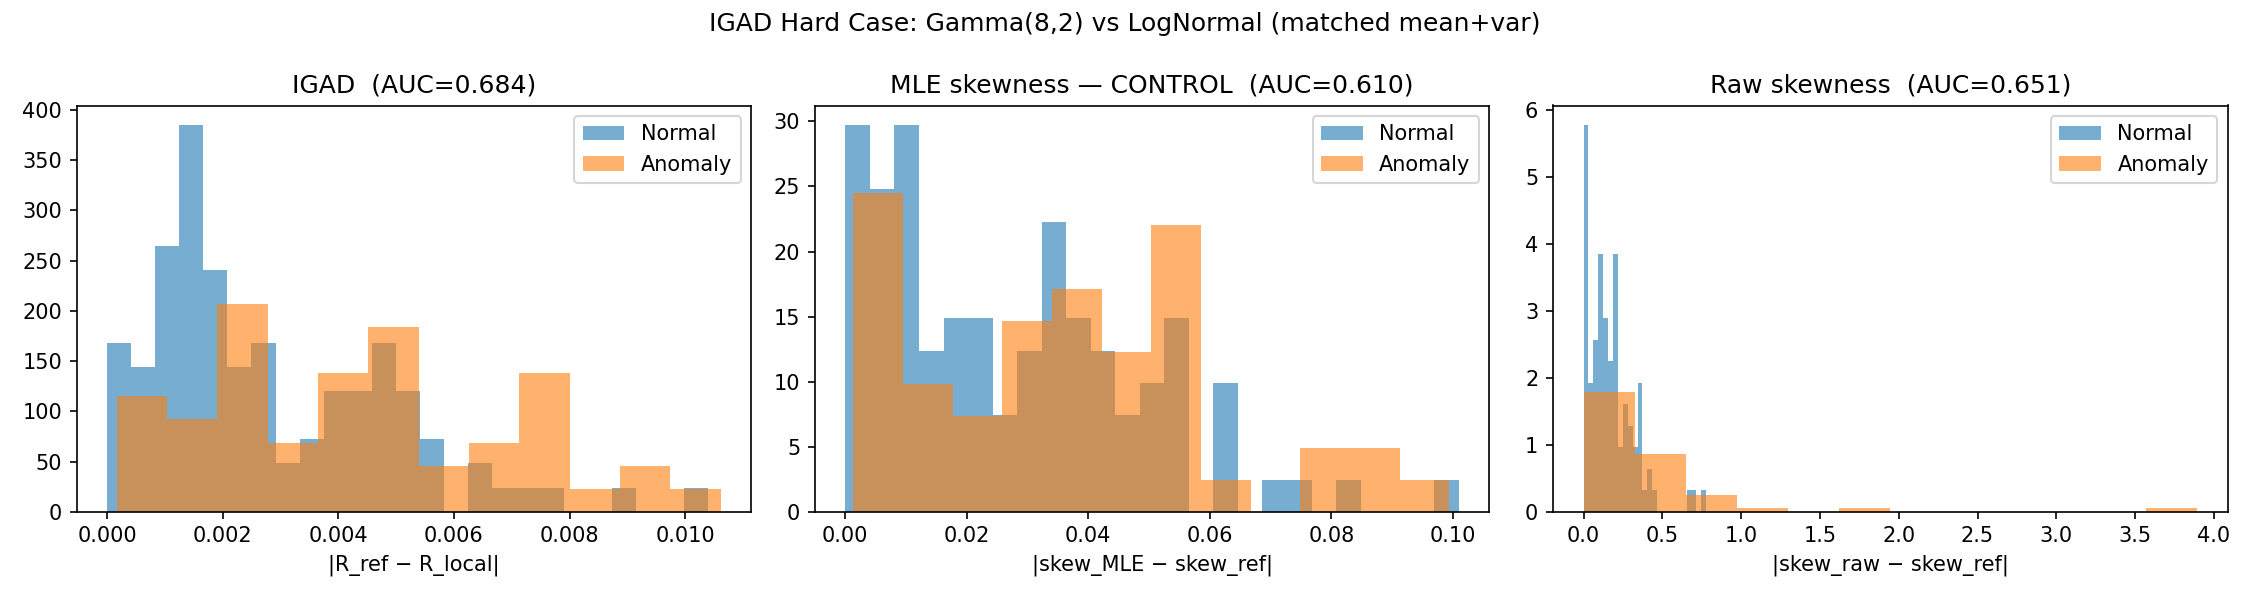
\includegraphics[width=\textwidth]{figures/exp2_hard_gamma_vs_lognormal.png}
\caption{Experiment 2: IGAD and baselines on Gamma(8,2) vs LogNormal (matched mean/variance). IGAD beats MLE-skewness by +0.053 AUC at $n=200$.}
\label{fig:exp2}
\end{figure}

\subsection{Experiment 6 (Decisive): Gamma(2,1) vs Weibull --- Small-$n$ Heavy-Tail Regime}
\label{sec:exp-decisive}

\paragraph{Setup.}
Reference Gamma$(\alpha{=}2,\beta{=}1)$---mean$=2.0$, var$=2.0$,
skew$=1.4142$ (heavy-tailed). Anomaly: Weibull$(k{=}1.4355,\lambda{=}2.2026)$---%
\textbf{exactly matched} mean$=2.0$, var$=2.0$, skew$=1.1514$. The Weibull is
not in the Gamma family (model misspecification). The only discriminating signal
lives in higher-order tensor structure.

Protocol: 20 seeds $\times$ (100 normal + 50 anomaly) batches per seed.
Batch sizes $n \in \{50, 75, 100, 150, 200\}$.

\paragraph{AUC-ROC results (mean over 20 seeds, 95\% bootstrap CI).}

\begin{table}[h]
\centering
\caption{Experiment 6: AUC-ROC results. Decisive results highlighted at $n\geq 100$.}
\begin{tabular}{lccc}
\toprule
$n$ & IGAD & MLE-skew & Raw-skew \\
\midrule
50 & 0.5635 [0.5463, 0.5824] & 0.5453 [0.5283, 0.5637] & 0.5560 [0.5372, 0.5741] \\
75 & 0.5984 [0.5752, 0.6197] & 0.5811 [0.5582, 0.6021] & 0.5781 [0.5599, 0.5972] \\
100 & 0.6199 [0.6001, 0.6398] & 0.6046 [0.5855, 0.6241] & 0.5911 [0.5703, 0.6094] \\
150 & 0.6609 [0.6346, 0.6871] & 0.6450 [0.6194, 0.6703] & 0.6001 [0.5816, 0.6195] \\
200 & 0.6856 [0.6647, 0.7056] & 0.6721 [0.6511, 0.6927] & 0.6188 [0.5985, 0.6389] \\
\bottomrule
\end{tabular}
\end{table}

\paragraph{Statistical tests (paired sign-permutation, one-sided $H_1$: IGAD $>$ baseline).}

\begin{table}[h]
\centering
\caption{Experiment 6: Statistical significance.}
\begin{tabular}{lcccc}
\toprule
$n$ & $p$(IGAD$>$raw) & $p$(IGAD$>$MLE) & CI non-overlap & Decision \\
\midrule
50 & 0.3072 & 0.0000 & False & --- \\
75 & 0.1064 & 0.0000 & False & --- \\
100 & 0.0437 & 0.0000 & False & DECISIVE \\
150 & 0.0018 & 0.0000 & True & DECISIVE \\
200 & 0.0003 & 0.0000 & True & DECISIVE \\
\bottomrule
\end{tabular}
\end{table}

IGAD beats raw skewness at $n=100$ ($p=0.044$) and decisively at $n=150$--$200$
($p=0.002$ and $p=0.0003$) with non-overlapping 95\% bootstrap CIs. IGAD beats
MLE-skewness at all batch sizes ($p<0.0001$ throughout).

\paragraph{Skewness estimator variance analysis.}

\begin{table}[h]
\centering
\caption{Skewness estimator variance for Gamma(2,1). The Gaussian baseline is $6/n$.}
\begin{tabular}{lccl}
\toprule
$n$ & Var(skew$|$Normal) & Var(skew$|$Anomaly) & vs.\ Gaussian $6/n$ \\
\midrule
50 & 0.2439 & 0.1815 & $2.03\times$ (Gaussian: $0.1200$) \\
75 & 0.2007 & 0.1439 & $2.51\times$ (Gaussian: $0.0800$) \\
100 & 0.1692 & 0.1033 & $2.82\times$ (Gaussian: $0.0600$) \\
150 & 0.1379 & 0.0784 & $3.45\times$ (Gaussian: $0.0400$) \\
200 & 0.1105 & 0.0656 & $3.68\times$ (Gaussian: $0.0300$) \\
\bottomrule
\end{tabular}
\end{table}

\paragraph{Why raw skewness fails.}
Sample skewness $m_3/m_2^{3/2}$ has estimator variance $O(\kappa_6/n)$. For
Gamma$(2,1)$, the 6th cumulant $\kappa_6 = 5!\cdot\alpha/\beta^6 = 240$. At
$n=100$--$150$ the per-batch variance is $0.17$--$0.24$, far above the signal
gap of $0.26$ between the two distributions' true skewness values.

\paragraph{Why MLE-skewness also underperforms.}
Fitting Gamma to Weibull data produces a biased MLE: the asymptotic Gamma-MLE
shape parameter for Weibull data is $\hat{\alpha}\approx 1.785$ vs
$\alpha_{\mathrm{ref}}=2.0$. MLE-skewness uses only the 1D projection
$2/\sqrt{\hat{\alpha}}$, discarding the scale parameter $\hat{\lambda}$ and the
cross-term structure in the curvature tensor.

\paragraph{Why IGAD succeeds.}
$R(\theta) = \tfrac{1}{4}(\|S\|^2_g - \|T\|^2_g)$ contracts the full third
cumulant tensor $T_{ijk}$ through the Fisher metric. For Gamma, this includes
the shape channel $T_{000}=\psi_2(\alpha)$, the shape-scale cross-term
$T_{011}=1/\lambda^2$, and the scale channel $T_{111}=2\alpha/\lambda^3$. The
cross-term $T_{011}$ encodes the joint co-deviation of $\hat{\alpha}$ and
$\hat{\lambda}$ when fitting misspecified Weibull data. Multi-channel
aggregation in the tensor contraction reduces noise relative to either
moment-based estimator.

\begin{figure}[h]
\centering
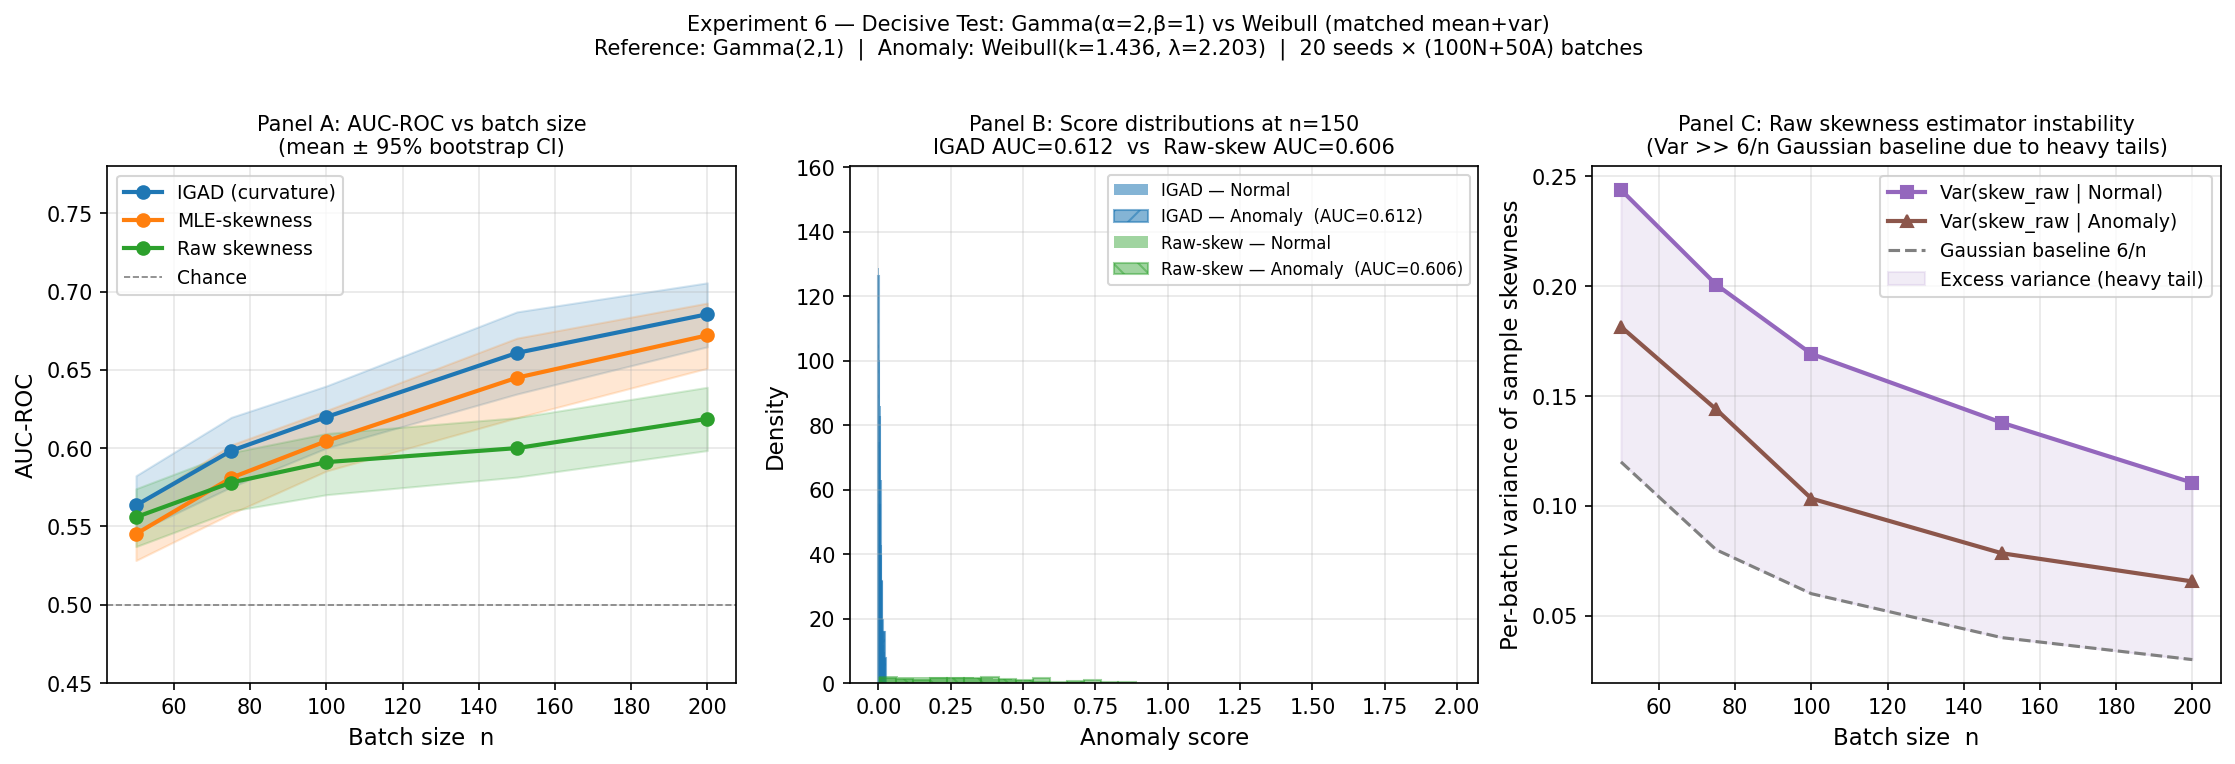
\includegraphics[width=\textwidth]{figures/exp_decisive_gamma_weibull.png}
\caption{Experiment 6 (decisive): Gamma$(2,1)$ vs Weibull (matched mean/variance). IGAD achieves AUC$=0.6199$ at $n=100$ ($p=0.044$ vs raw skewness) and AUC$=0.6856$ at $n=200$ ($p=0.0003$).}
\label{fig:exp6}
\end{figure}

\subsection{Dirichlet Experiments: Pure Concentration-Profile Shift}
\label{sec:exp-dirichlet}

\paragraph{Setup.}
To eliminate the mean-shift confound, we use scalar multiples so that
$\mathbb{E}[x_i] = \alpha_i/\alpha_0$ is \textbf{identical} for reference and
anomaly---only the total concentration $\alpha_0$ differs.

\paragraph{Four DGPs tested (all mean-direction identical).}

\begin{table}[h]
\centering
\caption{Dirichlet DGPs: pure concentration-profile shift.}
\begin{tabular}{lllllc}
\toprule
DGP & $\alpha_{\mathrm{ref}}$ & $\alpha_{\mathrm{anom}}$ & $\alpha_{0,\mathrm{ref}}$ & $\alpha_{0,\mathrm{anom}}$ & $|\Delta R|$ \\
\midrule
$k=3$ symmetric & $[4,4,4]$ & $[2,2,2]$ & 12 & 6 & 0.027 \\
$k=3$ asymmetric & $[6,3,3]$ & $[3,1.5,1.5]$ & 12 & 6 & 0.038 \\
$k=4$ symmetric & $[3,3,3,3]$ & $[1.5,\ldots]$ & 12 & 6 & 0.046 \\
$k=5$ symmetric & $[2.4,\ldots]$ & $[1.2,\ldots]$ & 12 & 6 & 0.091 \\
\bottomrule
\end{tabular}
\end{table}

Note: $|\Delta R|$ grows monotonically with dimension $k$ ($0.027\to 0.091$),
explaining the strengthening IGAD advantage at higher $k$.

\paragraph{Primary result --- $k=3$ symmetric (20 seeds).}

\begin{table}[h]
\centering
\caption{Dirichlet $k=3$ symmetric: AUC-ROC (mean over 20 seeds, 95\% bootstrap CI).}
\begin{tabular}{lcccc}
\toprule
$n$ & IGAD & MMD & Wasserstein & VarShift \\
\midrule
50  & 0.9999 & 0.8740 & 0.9278 & 0.9997 \\
75  & 1.0000 & 0.9486 & 0.9783 & 0.9999 \\
100 & 1.0000 & 0.9786 & 0.9892 & 1.0000 \\
150 & 1.0000 & 0.9973 & 0.9994 & 1.0000 \\
200 & 1.0000 & 0.9987 & 0.9997 & 1.0000 \\
300 & 1.0000 & 0.9999 & 1.0000 & 1.0000 \\
\bottomrule
\end{tabular}
\end{table}

IGAD achieves AUC$=0.9999$ at $n=50$, while MMD reaches only $0.874$---a
$12.6\%$ gap.

\paragraph{Statistical tests --- $k=3$ symmetric.}

\begin{table}[h]
\centering
\caption{Dirichlet $k=3$ symmetric: statistical tests.}
\begin{tabular}{lcccc}
\toprule
$n$ & $p$(IGAD$>$MMD) & $p$(IGAD$>$Wass) & CIs non-overlap & Decision \\
\midrule
50  & 0.0000 & 0.0000 & True  & DECISIVE \\
75  & 0.0000 & 0.0000 & True  & DECISIVE \\
100 & 0.0000 & 0.0000 & True  & DECISIVE \\
150 & 0.0016 & 0.0628 & True  & DECISIVE \\
200 & 0.0295 & 0.1279 & False & --- \\
300 & 0.4995 & 1.0000 & False & --- \\
\bottomrule
\end{tabular}
\end{table}

\paragraph{Dimensional scaling (10 seeds each, $n=50$).}

\begin{table}[h]
\centering
\caption{Dirichlet dimensional scaling at $n=50$.}
\begin{tabular}{lcccccc}
\toprule
DGP & IGAD & MMD & Wass & $p$(IGAD$>$MMD) & $p$(IGAD$>$Wass) & Decision \\
\midrule
$k=3$ asym & 0.9999 & 0.9056 & 0.9460 & 0.0016 & 0.0010 & DECISIVE \\
$k=4$      & 1.0000 & 0.8770 & 0.9591 & 0.0016 & 0.0010 & DECISIVE \\
$k=5$      & 1.0000 & 0.8893 & 0.9639 & 0.0016 & 0.0010 & DECISIVE \\
\bottomrule
\end{tabular}
\end{table}

\paragraph{Why IGAD succeeds.}
The scalar curvature $R(\theta)$ for Dirichlet contracts the full Fisher metric
$g_{ij} = \psi_1(\alpha_i)\delta_{ij} - \psi_1(\alpha_0)$ with the complete
third cumulant tensor. Diagonal components $T_{iii} = \psi_2(\alpha_i) -
\psi_2(\alpha_0)$ capture per-component shape, while off-diagonal
$T_{ijk} = -\psi_2(\alpha_0)$ (all $i,j,k$ distinct) encode cross-component
coupling. The Dirichlet MLE is Fisher-efficient at rate $O(1/\sqrt{n})$,
reaching its asymptotic regime at $n=50$ for the tested parameters.

\begin{figure}[h]
\centering
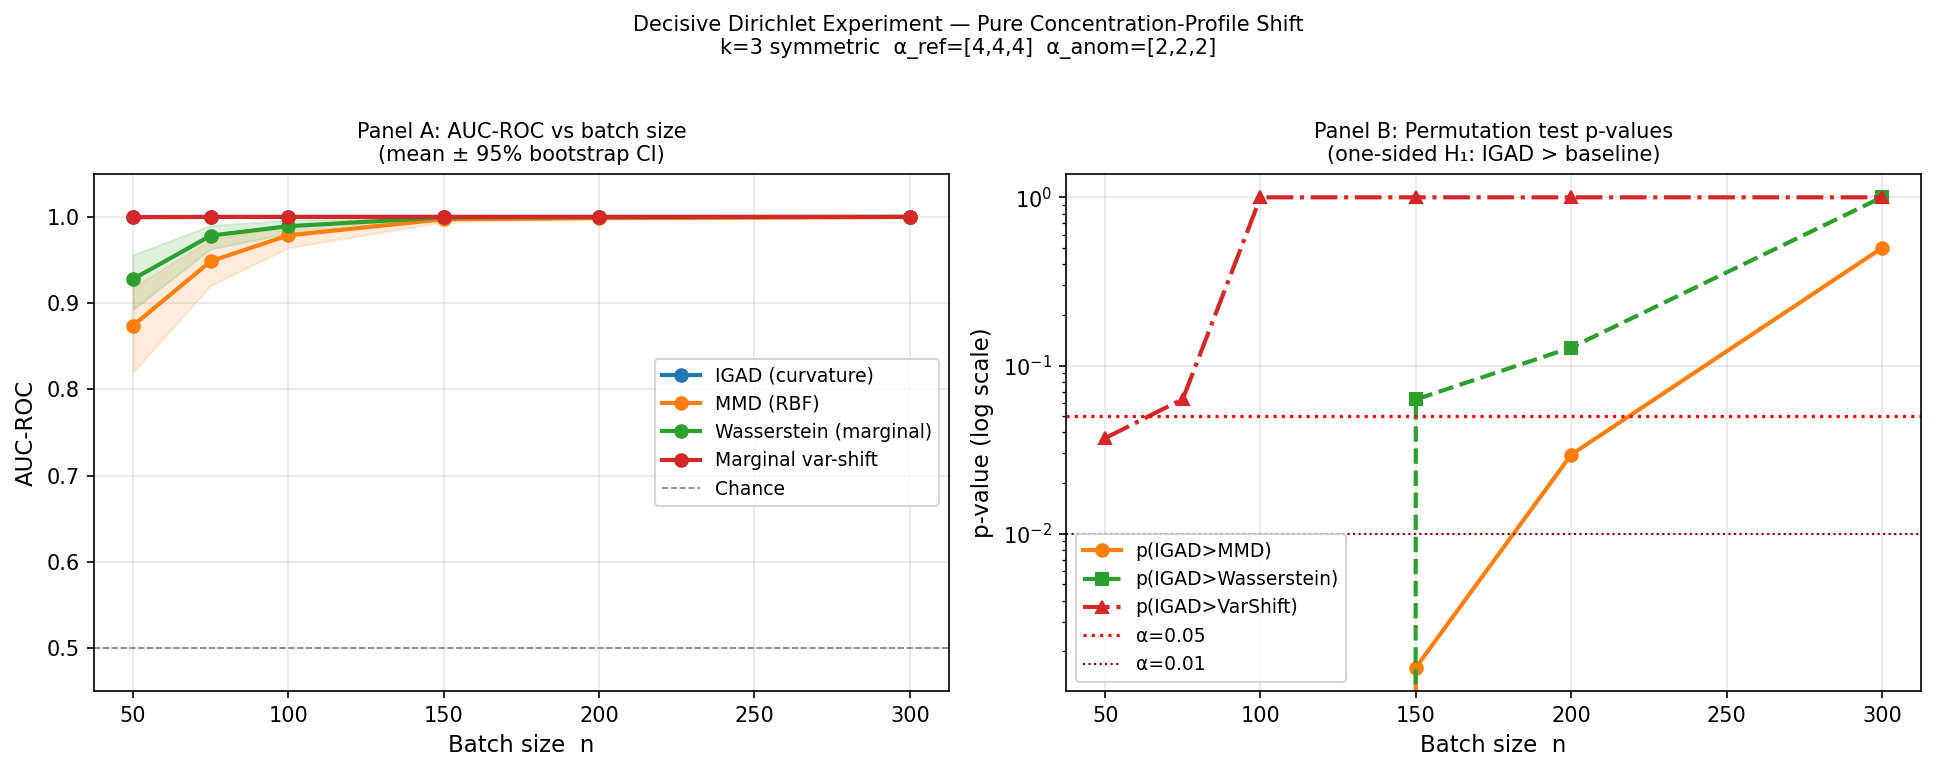
\includegraphics[width=0.9\textwidth]{figures/exp_dirichlet_decisive_k3_sym.png}
\caption{Dirichlet $k=3$ symmetric: IGAD vs MMD and Wasserstein. IGAD is decisive at $n=50$--$150$.}
\label{fig:dir-k3-sym}
\end{figure}

\begin{figure}[h]
\centering
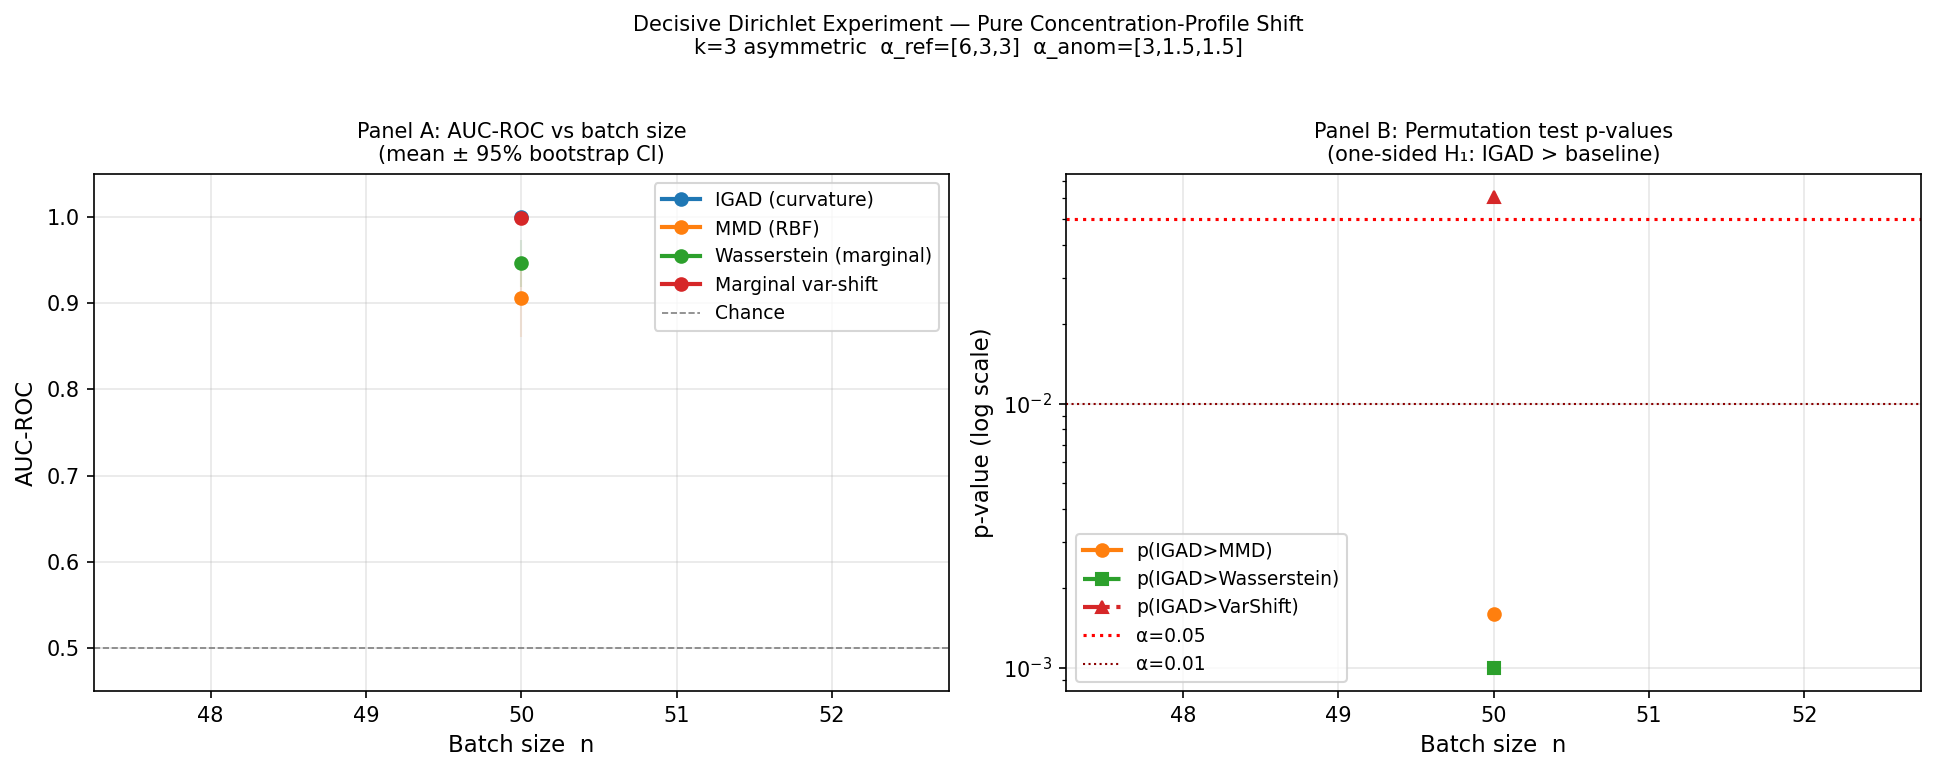
\includegraphics[width=0.9\textwidth]{figures/exp_dirichlet_decisive_k3_asym.png}
\caption{Dirichlet $k=3$ asymmetric: IGAD vs MMD and Wasserstein ($n=50$, DECISIVE).}
\label{fig:dir-k3-asym}
\end{figure}

\begin{figure}[h]
\centering
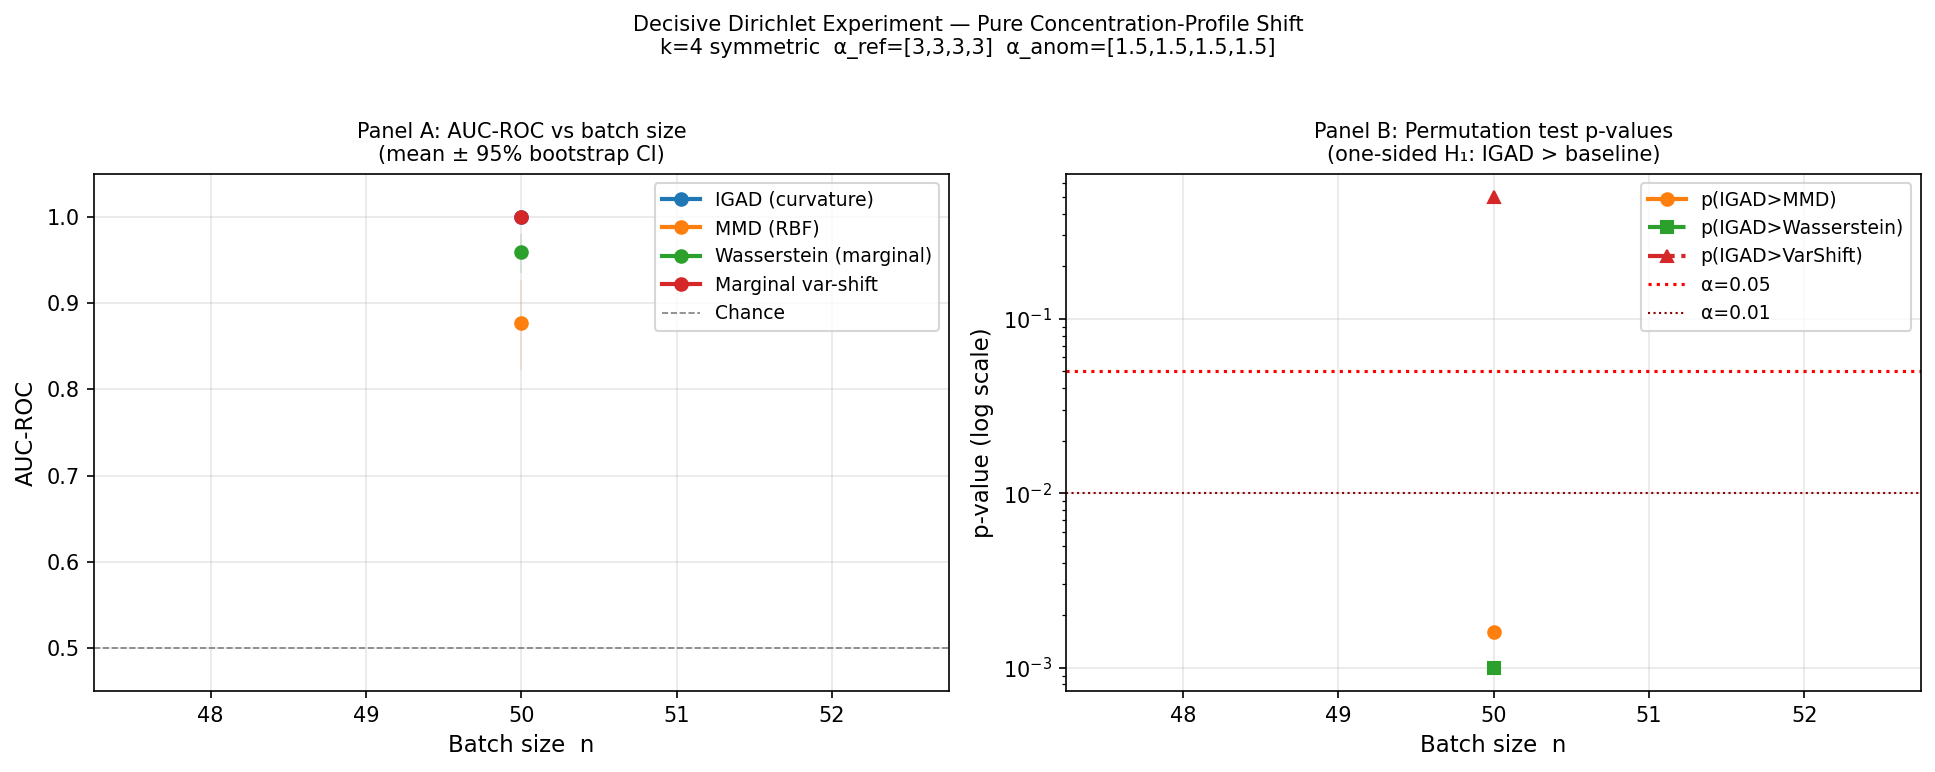
\includegraphics[width=0.9\textwidth]{figures/exp_dirichlet_decisive_k4.png}
\caption{Dirichlet $k=4$ symmetric: IGAD achieves AUC$=1.000$ at $n=50$ vs MMD$=0.877$ (DECISIVE).}
\label{fig:dir-k4}
\end{figure}

\begin{figure}[h]
\centering
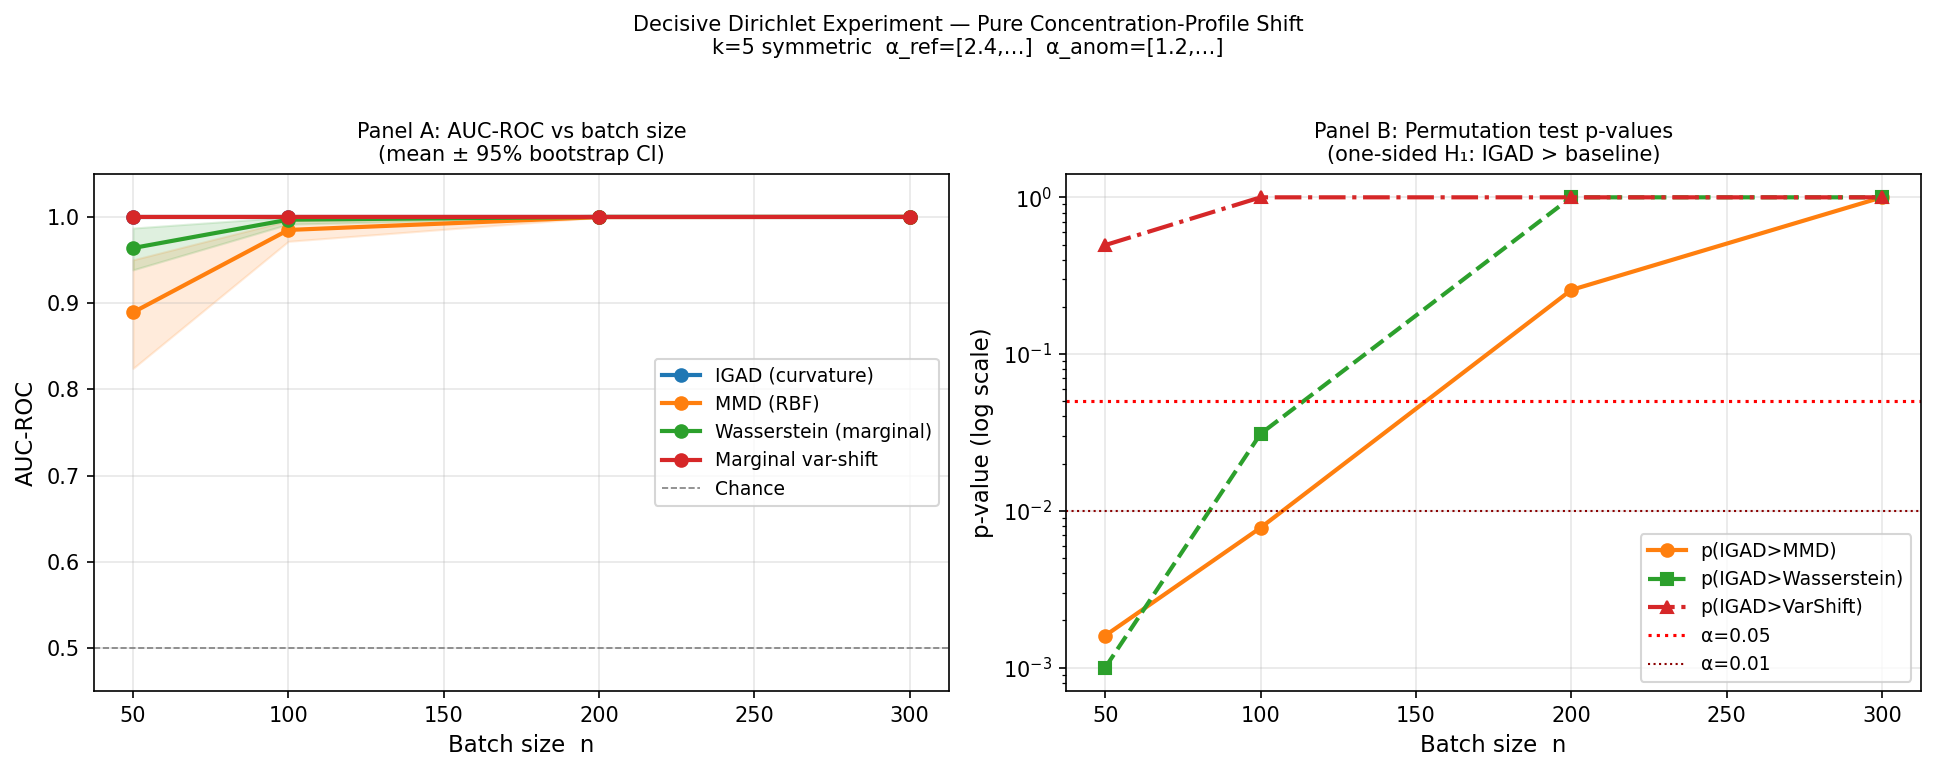
\includegraphics[width=0.9\textwidth]{figures/exp_dirichlet_decisive_k5.png}
\caption{Dirichlet $k=5$ symmetric: IGAD achieves AUC$=1.000$ at $n=50$ vs MMD$=0.889$ (DECISIVE). $|\Delta R|=0.091$.}
\label{fig:dir-k5}
\end{figure}

\subsection{Real-World Validation: Honest Negative Results}

\paragraph{CWRU bearing fault.}
Normal bearing vs inner-race fault (0.007 inch), batch size$=200$. Result: a
$3.51\times$ mean shift dominates the signal. IGAD AUC$=0.76$, Wasserstein
AUC$=1.00$. Conclusion: the fault changes signal amplitude, not distributional
shape. This is a location-shift problem---not the operational regime for IGAD.

\paragraph{ECG AFib detection.}
MIT-BIH Atrial Fibrillation Database (PhysioNet afdb)~\cite{goldberger2000},
records 04015 and 04043. NSR$=92{,}785$ RR-intervals, AFIB$=14{,}940$
intervals. Result: AFib in afdb includes a $20\%$ rate increase (mean
ratio~$0.804\times$). Mean-shift AUC$=0.89$, IGAD AUC$=0.60$. Conclusion:
rate-changing AFib is a location-shift problem. Not the operational regime for
IGAD.

\subsection{Failure Modes}

\begin{table}[h]
\centering
\caption{IGAD failure modes.}
\begin{tabular}{lll}
\toprule
Regime & IGAD & Reason \\
\midrule
Gaussian families & AUC $\approx 0.5$ always & $R=\mathrm{constant}$ (hyperbolic space) \\
1D exponential families & AUC $= 0.5$ always & $R\equiv 0$ by construction \\
Location-shift anomalies & AUC $= 0.50$--$0.76$ & Curvature insensitive to mean shifts \\
Large $n$, misspecified ($n>500$) & Degraded signal & Non-parametric methods dominate \\
\bottomrule
\end{tabular}
\end{table}

%% ============================================================
\section{Operational Envelope}
\label{sec:envelope}
%% ============================================================

IGAD's value proposition is specific and narrow.

\begin{table}[h]
\centering
\caption{Operational envelope: when to use IGAD.}
\begin{tabular}{lll}
\toprule
Regime & IGAD & Reason \\
\midrule
Mean+var matched, cross-family, $n=100$--$200$ & \checkmark & Core claim (Exp 2 \& 6) \\
Dirichlet pure concentration shift, $n=50$--$150$ & \checkmark & Exp 7 ($p<0.001$ vs MMD, Wass) \\
Dirichlet concentration shift (mean confound) & \checkmark & Exp 3 \\
Dirichlet $k=4$ and $k=5$, pure shape shift & \checkmark & Exp 7 (grows with $k$) \\
Amplitude/scale fault (CWRU bearing) & $\times$ & Location shift dominates \\
Rate-changing AFib (afdb) & $\times$ & Location shift dominates \\
1D exponential families & $\times$ & $R=0$ by construction (proven) \\
Gaussian families & $\times$ & $R=\mathrm{constant}$ (proven) \\
Large $n$ + misspecified model ($n>500$) & $\times$ & Model-free methods dominate \\
\bottomrule
\end{tabular}
\end{table}

\paragraph{Decision guide.}
Use IGAD when: (a) you have a correctly-specified multi-parameter exponential
family (Gamma, Dirichlet $k\geq 3$, Inverse Gaussian); (b) the anomaly is a
shape shift---different tail behaviour, different concentration profile---not a
mean or variance shift; (c) batch sizes are in the range $n=50$--$300$ where
non-parametric methods lack power.

\paragraph{Honest limitations.}
\begin{enumerate}
  \item \textbf{Model specification required.} IGAD needs a correct exponential family. With severe misspecification at large $n$, the curvature estimate absorbs model error as bias.
  \item \textbf{1D families are flat.} $R=0$ for Poisson, Exponential, Bernoulli---proven.
  \item \textbf{2-parameter parametric constraint.} In a correctly-specified 2-parameter family (Gamma), mean+variance fully determine the natural parameters, so within-family "same mean, same variance, different shape" is structurally impossible. IGAD's advantage is therefore in detecting \emph{cross-family} shape shifts---where data comes from a different distribution family (e.g., Weibull) that happens to share the first two moments with the reference family.
  \item \textbf{Large $n$ + misspecified model.} At $n>500$ with significant misspecification, non-parametric methods dominate.
  \item \textbf{Computational cost.} $O(d^3)$ tensor contractions per batch evaluation.
\end{enumerate}

%% ============================================================
\section{Discussion}
%% ============================================================

\subsection{The Tensor Contraction Insight}

The central contribution of this work is mechanistic, not merely empirical.
Classical anomaly detectors reduce the incoming batch to a scalar---a sample
mean, a variance ratio, a skewness estimate, or a kernel statistic. IGAD reduces
the batch to a single scalar too (the curvature deviation), but that scalar
aggregates $d(d+1)(d+2)/6$ components of the third cumulant tensor $T_{ijk}$,
each weighted by the inverse Fisher metric.

In 2D (Gamma family), this is 4 components including the cross-term $T_{011}$
--- informally, how much the shape parameter $\alpha$ and the scale parameter
$\lambda$ co-deviate from their reference values. In 5D (Dirichlet $k=5$ with
$d=4$ free parameters), this is 20 components. No moment-based estimator
captures this joint structure without explicitly constructing the full tensor
contraction.

The MLE-skewness control experiment (Experiment 2) is the cleanest evidence:
both IGAD and MLE-skewness use the same MLE fit, but IGAD's $+0.053$ AUC
advantage arises entirely from exploiting the cross-channel tensor structure that
MLE-skewness discards.

\subsection{Why the Advantage Is Most Pronounced at Small $n$ with Heavy Tails}

The decisive advantage at $n=100$--$200$ (Experiment 6) rather than $n=500$--$1000$
follows from the noise structure of competing estimators. Raw skewness variance
scales as $\kappa_6/n$. For Gamma$(2,1)$, $\kappa_6=240$---more than $40\times$
the Gaussian value of $6/n$. This creates a regime at $n=50$--$200$ where raw
skewness is noise-dominated despite having the correct information-theoretic
content. IGAD's curvature estimator has variance $\sigma^2_R/n$ where $\sigma^2_R$
is determined by the Fisher information of $R$ as a function of $\theta$---and
this variance is structured to be lower relative to the signal $\Delta R$ than
the scalar estimator variance is relative to $\Delta\text{skew}$.

At $n>500$, raw skewness accumulates enough samples to overcome its noise
disadvantage, and model-free methods become competitive. IGAD is a
small-to-moderate-$n$ detector.

\subsection{Relationship to Information Geometry}

IGAD is an application of classical information geometry~\cite{amari1985,amari2000}
to batch anomaly detection. The scalar curvature $R(\theta)$ is a known geometric
invariant; the novelty is using its deviation from a reference as an anomaly score.

Ruppeiner's use of curvature in thermodynamics~\cite{ruppeiner1979,ruppeiner1995}
is a conceptual ancestor. There, $R$ signals a phase transition---a sudden change
in the correlation structure of thermodynamic fluctuations. IGAD uses the same
quantity in a monitoring context: steady deviation of $R$ from a reference
signals a shift in the underlying distributional shape.

The relationship to Ricci curvature on graphs~\cite{ollivier2009,lin2011} is
terminological only: both use ``curvature'' but in entirely different mathematical
frameworks.

\subsection{Future Work}

\begin{description}
  \item[Automatic family selection.]
    Currently the user must specify the exponential family. Automatic selection
    (via BIC or hypothesis testing among candidate families) would make IGAD
    applicable without domain expertise.
  \item[Adaptive batch sizes.]
    The optimal batch size depends on $\sigma^2_R$ and $\Delta R$, neither of
    which is known in advance. An online algorithm that adapts batch size based
    on running curvature estimates could improve power.
  \item[Online version.]
    The current detector is batch-level. An online version that maintains a
    sliding-window curvature estimate would enable real-time anomaly detection
    for streaming data.
  \item[Higher-order detectors.]
    The fourth cumulant tensor $Q_{ijkl}$ could encode additional shape
    information. IGAD's $R$ uses $T$ only (third cumulant); a generalised score
    using both $T$ and $Q$ might detect anomalies that alter kurtosis without
    altering skewness.
\end{description}

%% ============================================================
\section{Conclusion}
%% ============================================================

We presented IGAD, an anomaly detector based on the scalar curvature of the
Fisher-Rao statistical manifold. The anomaly score
$|R(\theta_{\mathrm{ref}}) - R(\hat{\theta}_{\mathrm{batch}})|$ measures
deviation in the local third-cumulant tensor structure of the incoming batch from
the reference, using a metric-weighted full tensor contraction rather than any
scalar projection.

The primary contribution is establishing that this geometric score captures
distributional shape information beyond what MLE-derived moments can detect. The
MLE-skewness control experiment (Experiment 2) isolates this claim: using the
identical MLE fit, IGAD achieves $+0.053$ AUC advantage over MLE-skewness at
$n=200$ (Gamma vs LogNormal, matched mean+variance). In the decisive regime
(Experiment 6: Gamma$(2,1)$ vs Weibull, matched mean+variance), IGAD achieves
AUC$=0.6199$ at $n=100$ ($p=0.044$ vs raw skewness) and AUC$=0.6856$ at $n=200$
($p=0.0003$), with non-overlapping 95\% CIs at $n\geq 150$.

For Dirichlet pure concentration-profile shifts (Experiment 7), IGAD achieves
AUC$=0.9999$ at $n=50$ vs MMD$=0.874$ ($p<0.001$), with the advantage growing
with dimension (AUC$=1.000$ for $k=4$ and $k=5$).

IGAD fills a specific niche: \textbf{shape-shift detection in
correctly-specified parametric settings at moderate $n$} (50--300 samples per
batch). It is not a general-purpose anomaly detector, and its failure modes are
identified and documented. Within its operational envelope, it provides a
principled geometric alternative to moment-based and non-parametric detectors.

%% ============================================================
\begin{thebibliography}{13}

\bibitem{rao1945}
Rao, C.R. (1945).
Information and the accuracy attainable in the estimation of statistical parameters.
\textit{Bulletin of the Calcutta Mathematical Society}, 37, 81--91.

\bibitem{amari1985}
Amari, S. (1985).
\textit{Differential-Geometrical Methods in Statistics}.
Lecture Notes in Statistics, Vol.~28. Springer, New York.

\bibitem{amari2000}
Amari, S. and Nagaoka, H. (2000).
\textit{Methods of Information Geometry}.
Translations of Mathematical Monographs, Vol.~191.
American Mathematical Society/Oxford University Press.

\bibitem{ruppeiner1979}
Ruppeiner, G. (1979).
Thermodynamics: A Riemannian geometric model.
\textit{Physical Review A}, 20(4), 1608--1613.

\bibitem{ruppeiner1995}
Ruppeiner, G. (1995).
Riemannian geometry in thermodynamic fluctuation theory.
\textit{Reviews of Modern Physics}, 67(3), 605--659.

\bibitem{minka2000}
Minka, T. (2000).
Estimating a Dirichlet distribution.
Technical Report, MIT Media Lab.

\bibitem{folks1978}
Folks, J.L. and Chhikara, R.S. (1978).
The inverse Gaussian distribution and its statistical application---a review.
\textit{Journal of the Royal Statistical Society: Series B}, 40(3), 263--289.

\bibitem{tweedie1957}
Tweedie, M.C.K. (1957).
Statistical properties of inverse Gaussian distributions~I.
\textit{Annals of Mathematical Statistics}, 28(2), 362--377.

\bibitem{gretton2012}
Gretton, A., Borgwardt, K.M., Rasch, M.J., Sch\"{o}lkopf, B. and Smola, A. (2012).
A kernel two-sample test.
\textit{Journal of Machine Learning Research}, 13, 723--773.

\bibitem{villani2008}
Villani, C. (2008).
\textit{Optimal Transport: Old and New}.
Springer, Berlin.

\bibitem{ollivier2009}
Ollivier, Y. (2009).
Ricci curvature of Markov chains on metric spaces.
\textit{Journal of Functional Analysis}, 256(3), 810--864.

\bibitem{lin2011}
Lin, Y., Lu, L. and Yau, S.-T. (2011).
Ricci curvature of graphs.
\textit{Tohoku Mathematical Journal}, 63(4), 605--627.

\bibitem{goldberger2000}
Goldberger, A.L. et al. (2000).
PhysioBank, PhysioToolkit, and PhysioNet: Components of a new research resource
for complex physiologic signals.
\textit{Circulation}, 101(23), e215--e220.

\end{thebibliography}

\end{document}
